\section{Højtaler}

For at kunne sammenligne teori og praksis, kan højtaler-dataen fra tabel \ref{tab:TS} benyttes til at udformere et simuleret frekvensrespons, ud fra de forskellige portlængder på basrefleksen. 

Ved at beregne volumenhastigheden for den elektriske impedans, kan man opdele bidraget fra fronten af højtaleren, samt for porten, for til sidst at lave det samlede tryk til en ønsket afstand. 


\subsection{Volumenhastighed Front:}
\label{sec:sim_calc}

Ud fra impedansen af det samlede system, kan volumenhastigheden for højtalerenheden i kabinettet beregnes. Dette er hastigheden af det volumen af luft som skubbes foran højtaleren. 

{\Large\(qF=\)}{\huge \(\frac{F_A}{R_{AE}+s*M_{AS}+\frac{1}{s*C_{AS}}+Ras+\frac{1}{(s*C_{AB}+\frac{1}{s*M_{AP}}}}\) }

I denne beregning, indgår også \textit{massen af luften i porten} ($M_{AP})$, som beror sig på radius af porten og længden af porten:\\

\(M_{AP}=\frac{(\rho)}{S_P}*(L_P+1.46*\sqrt{\frac{S_P}{\pi}}\))

Da kabinettet i projektet allerede var konstrueret med en enkelt port, er radius af porten fastsat fra start.

\(r_P=0.025 m\)		\hspace{6.2cm} Portens Radius\\
\(S_P=\pi*r_P^2=pi*0.025^2=0.0020 m^2\)		\hspace{2cm} Portens overfladeareal\\

\(L_P=\frac{\gamma*P_0}{\rho*(2*\pi*f_p)^2*V_{B}}-1.46\sqrt{\frac{S_P}{\pi}}\)			\hspace{3cm} Hvor $\gamma \approx 1.4$ \& $P_0=100*10^3)$\\

Dermed får vi den optimale portlængde:\\

\(L_P=\frac{1.4*100*10^3}{1.18*(2*\pi*44)^2*16.5*10-3}-1.46\sqrt{\frac{0.0020}{\pi}}=15cm\)


\subsection{Volumenhastighed Port:}

Ovenpå at beregne volumenhastigheden for højtalerenheden, beregnes bidraget fra porten ud fra følgende formel:

{\Large\(qP=-qF*\)}{\huge \(\frac{\frac{1}{s*C_{AB}}}{\frac{1}{s*C_{AB}}+s*M_{AP}}\) }
\fxnote{s 61 Tores bog}


\subsection{Beregning af samlet lydtryk:}

For at omregne de to volumenhastigheder til et lydtryk i afstanden \textit{r}, benyttes følgende formel:

\(L=20*log_{10}(\frac{\frac{\rho*f}{r}*(qF+qP)}{pRef}) dB SPL\)

\fixme{Start mere generelt. Mere teori om lydm før vi angriber enheden. Mere teori om impedans-tilpasningen - AB}
Højtaleren der benyttes til projektet er en 6.5" mellemtone elektrodynamisk højtaler af mærket FW168\cite{FW168} fra firmaet Fountek \cite{Fountek}. 

På figur \ref{fig:kompletmodel} ses den komplette model for højtalerens elektriske, mekaniske og akustiske system.\citep{Elektroakustik} Komponentværdierne og forklaringen af disse, kan ses i tabel \ref{tab:TS}.

\begin{figure}[H]
	\centering
	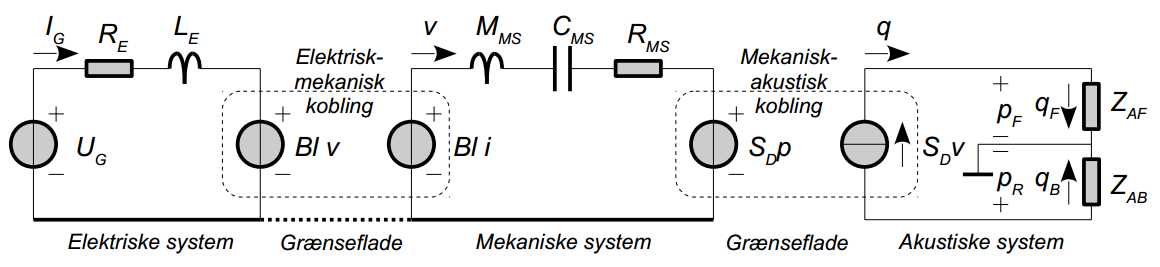
\includegraphics[width=\textwidth]{Pics/kompletmodel.PNG}
	\label{fig:kompletmodel}
	\caption{Komplet model fro højtalerens elektrisk, mekaniske- og akustiske system. } 
\end{figure}

\begin{table}
	\centering
	\begin{tabular}[C]{|c|c|c|}
		
		
		\hline	
		\textbf{Thiele-Small parameter} & \textbf{Symbol} & \textbf{Værdi for FW168} \\\hline
		Svingspolens DC modstand & $R_E$ & $7.2\Omega$ \\\hline
		Svingspolens selvinduktion & $L_E$ & $1mH$  \\\hline
		Elektrisk godhed & $Q_{ES}$ & 0.452 \\\hline
		Masse af bevægeligt system & $M_{MS}$ & $14.7g$  \\\hline
		Eftergivelighed af styr & $C_{MS}$ & $0.821mm/N$  \\\hline
		Mekanisk godhed & $Q_{MS}$ & 3.246  \\\hline
		Mekanisk tabsmodstnd & $R_{MS}$ & \( \frac{1}{Q_{MS}}\sqrt{\frac{M_{MS}}{C_{MS}}}=1.304Ns/m \)  \\\hline
		Resonansfrekvens & $f_s$ & \( \frac{1}{2\pi\sqrt{M_{MS} C_{MS}}}=45.813Hz \) \\\hline
		
		
		Ækvivalent volumen & $ V_{AS} $ & $16.5L=0.017m^3$ \\\hline
		Kraftfaktor & $Bl$ & $8.2Tm$ \\\hline
		Membranens effektive areal & $S_D$ & $119cm^2$ \\\hline
		Maksimal lineær bevægelse & $X_{MAX}$ & $4.6mm\pm$ \\\hline
		
	\end{tabular}
	\label{tab:TS}
\end{table}

Omregner man modellen til en komplet elektrisk model, kan man udregne den elektriske impedans $Z_E$ for modellen. Denne impedans har et toppunkt ved højtalerens resonansfrekvens, og en minimumsværdi ved svingspolens $R_E$-værdi. \fixme{Men hvorfor er det vigtigt? Teorien bag! - AB}

Med værdierne fra tabel \ref{tab:TS}, som er opgivet i højtalerens datablad\cite{FW168}, udregnes den elektriske impedans for højtaleren i ligning \ref{eq:eq1}

\begin{equation}\label{eq:eq1}
	Z_E(s)=R_E+sL_E+\frac{Bl^2}{\omega_s M_{MS}} \frac{ \omega_s s}{ s^2 + \frac{1}{Q_{MS}} \omega_s s + \omega_s^2} \end{equation} \begin{equation} \ \qquad  = 
	7.2\Omega + s \cdot 1mH + \frac{(8.2 Tm)^2}{287.8Hz \cdot 14.7gm} \frac{ 287.8Hz \cdot s}{ s^2 + \frac{1}{3.246} 287.8Hz \cdot s + (287.8Hz)^2}  \end{equation}

Impedansen vil være størst ved højtalerensresonansfrekvens $f_s$, som beregnes i ligning \ref{eq:fs}. Dette toppunkts maksimumværdi er givet ved ligning \ref{eq:Zmax} 

\begin{equation}\label{eq:fs}
	f_s=\frac{1}{2 \pi \sqrt{M_{MS} C_{MS}}}=45.813Hz
\end{equation}

\begin{equation}\label{eq:Zmax}
	Z_{max}=R_E+\frac{Bl^2}{R{MS}}=58.781\Omega
\end{equation}

På figur \ref{fig:ZE_graf} \fixme{Find ud af at lave det i matlab!!!! LS} ses plottet af ligning \ref{eq:eq1} med værdierne for højtaleren. Kurveforløbet stemmer overens med det beregnede toppunkt $f_s$ og minimumsværdien $R_E$. Kurveforløbet stemmer ligeledes overens med det opgivne i databladet \citep{FW168}.

\begin{figure}[H]
	\centering
	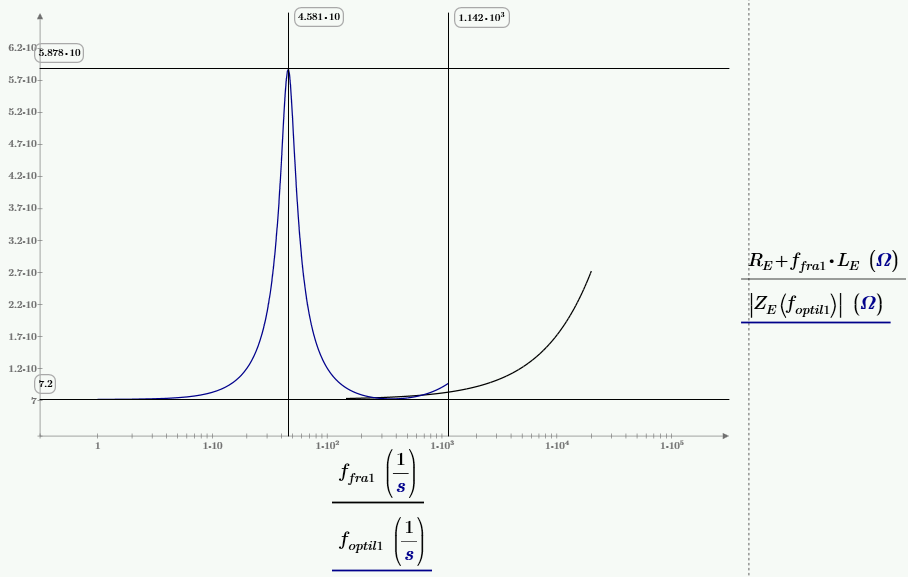
\includegraphics[width=\textwidth]{Pics/ZE_graf.PNG}
	\label{fig:ZE_graf}
	\caption{Den elektriske impedans $Z_E$ som funktion af frekvensen} 
\end{figure}
